%!TEX root = ../Main.tex
\begin{figure}
  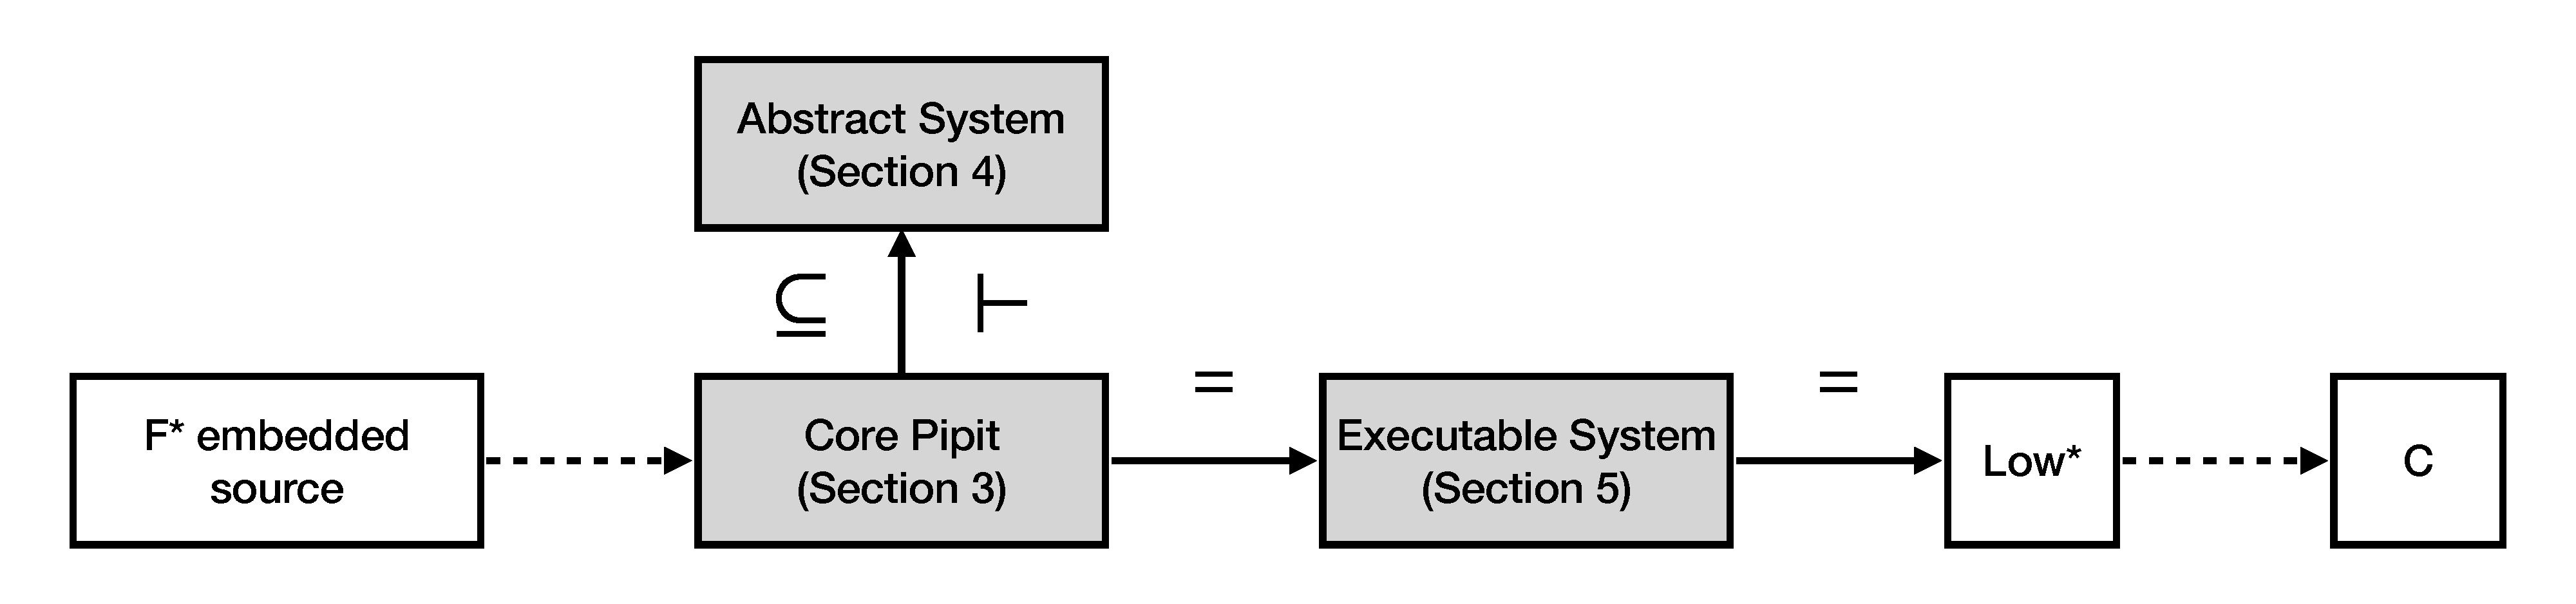
\includegraphics[width=\textwidth]{figures/core-structure-1920x450.pdf}
\caption{Architecture of Pipit. The gray boxes and solid arrows are defined in this paper. The white boxes and dashed arrows are trusted components. The labels denote verified properties of the translation: abstraction~($\subseteq$), entailment of proof obligations~($\vdash$), and equivalence~($=$).
}
\label{f:core:structure}
\end{figure}
